\ylDisplay{Klaaskuup} % Ülesande nimi
{Tundmatu autor} % Autor
{piirkonnavoor} % Voor
{2009} % Aasta
{G 7} % Ülesande nr.
{5} % Raskustase
{
% Teema: Geomeetriline-optika
\ifStatement
Klaaskuubi neli tahku on värvitud mustaks nõnda,
et värvimata jäänud tahud paiknevad kõrvuti (omavad ühist serva). Missugune peab olema klaasi murdumisnäitaja $n$, et ka värvimata tahud
paistaksid mustadena?
\fi


\ifHint
Mustaks värvitud tahkudelt valgus peegelduda ei saa, toimub neeldumine. Ülesande tingimus on täidetud, kui värvimata tahust kuupi sisenev valgus ei saa
väljuda läbi kõrvaltahu (toimub sisepeegeldus).
\fi


\ifSolution
Mustaks värvitud tahkudelt valgus peegelduda ei saa, toimub neeldumine. Ülesande tingimus on täidetud, kui värvimata tahust kuupi sisenev valgus ei saa
väljuda läbi kõrvaltahu (toimub sisepeegeldus). Sisepeegelduse kriitilise nurga saame murdumisseadusest:
\[
\sin \gamma_{C}=\frac{1}{n}.
\]

\begin{center}
	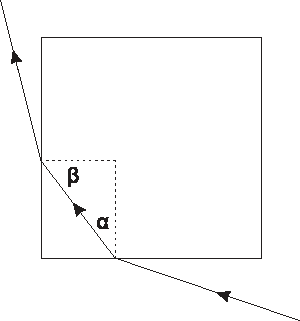
\includegraphics[width=0.45\linewidth]{2009-v2g-07-lah}
\end{center}

Kiir siseneb kuupi, kui $\alpha<\gamma_{C}$. Langemisnurk kõrvaltahule on $\beta = \SI{90}{\degree} - \alpha$. Kiir väljub kuubist, kui
\[
\beta<\gamma_{C}, \quad \text { ehk } \quad \SI{90}{\degree}<\gamma_{C}+\alpha<2 \gamma_{C}.
\]
Et kiir ei saaks kuubist väljuda, peab kehtima:
\[
\gamma_{C}<\SI{45}{\degree}, \quad \text { ehk } \quad n>1 / \sin \SI{45}{\degree}=\sqrt{2}.
\]
\fi
}